\section{Relative Entropy and Mutual Information}
概率论衡量两个变量相关程度(概率论方法):
$$\rho_{X,Y}=\dfrac{\Cov(X,Y)}{\sqrt{\Var(X)\Var(Y)}}\in[-1,1]$$
只能刻画\textbf{线性}相关性, 且正负相关程度相同(正负相关).

\begin{proposition}
$X$,$Y$独立, 则$\rho_{X,Y}=0$. 但是$\rho_{X,Y}=0$\textbf{不一定}独立.

\textcolor{red}{Gaussian分布独立$\Leftrightarrow$不相关}.
\end{proposition}

信息论衡量方法(用bit衡量):
\begin{definition}
$I(X;Y)$: $X$,$Y$之间的互信息(mutual information).
$$I(X;Y)=\sum_{x,y}p(x,y)\log\dfrac{p(x,y)}{p(x)p(y)}$$
\end{definition}

\begin{figure}[htbp]
    \centering
    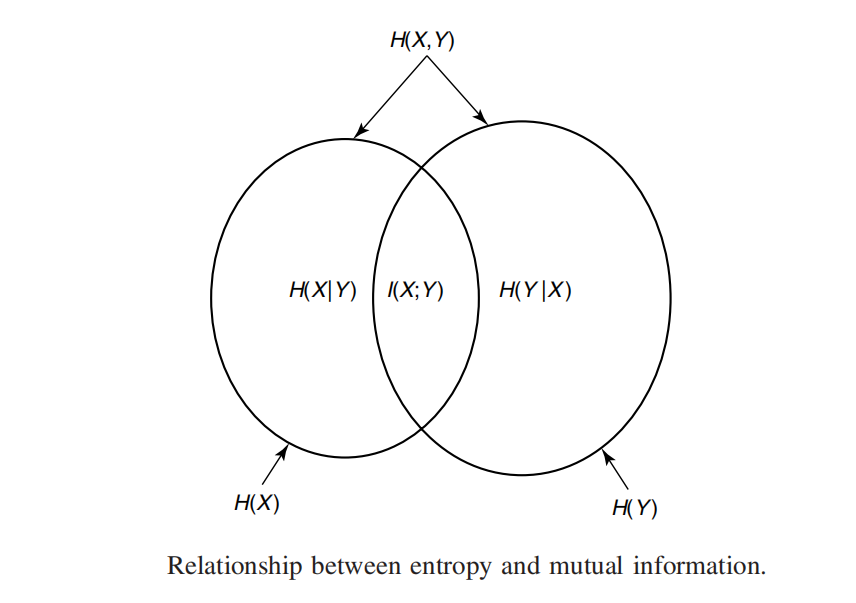
\includegraphics[width=0.83\textwidth]{./figures/chapter1/entropy_mutual_imformation.png}
\end{figure}

\begin{align*}
\textcolor{red}{H(X,Y)} &\ \textcolor{red}{= H(X) + H(Y|X)} \\
I(X;Y) &= H(X) - H(X|Y) \\
&= H(Y) - H(Y|X) \\
&= H(X) + H(Y) - H(X,Y)
\end{align*}

proof:
\begin{align*}
I(X;Y) &= \sum_{x,y}p(x,y)\log\dfrac{p(x,y)}{p(x)p(y)} \\
&= \sum_{x,y}p(x,y)\log\dfrac{p(x|y)p(y)}{p(x)p(y)} \\
&= \sum_{x,y}p(x,y)\log\dfrac{p(x|y)}{p(x)} \\
&= \sum_{x,y}p(x,y)\log\dfrac{1}{p(x)} - \sum_{x,y}p(x,y)\log\dfrac{1}{p(x|y)} \\
&= \sum_{x}p(x)\log\dfrac{1}{p(x)} - H(X|Y) \text{\ \ ($p(x,y)$对$y$求和,求出margin distribution $p(x)$)}\\
&= H(X) - H(X|Y)
\end{align*}

\begin{definition}
两个分布$p(x),q(x)$的相对熵 Relative Entropy(KL-Divergence):
$$D\left(p(x)\|q(x)\right)=\sum_{\textcolor{red}{x\in\mathcal{X}}}p(x)\log\dfrac{p(x)}{q(x)}$$
$\textcolor{red}{x\in\mathcal{X}}$: 不考虑两个support不同的分布.\\
物理意义: 两个分布之间的距离.
\end{definition}

\begin{proposition}
$D\left(p(x)\|q(x)\right)\geq 0$.\\
proof:
\begin{align*}
-D\left(p(x)\|q(x)\right) &= \sum_{x}p(x)\log\dfrac{q(x)}{p(x)} \\
&= \mathbb{E}_{x\sim p(x)}\left[\log\dfrac{q(x)}{p(x)}\right] \\
&\leq \log\mathbb{E}_{x\sim p(x)}\left[\dfrac{q(x)}{p(x)}\right] \textcolor{red}{\text{\ \ \ \ (Jensen's Inequality)}} \\
&= \log\sum_{x}p(x)\dfrac{q(x)}{p(x)} \\
&= 0
\end{align*}
i.e. $D\left(p(x)\|q(x)\right)\geq 0$.\\
当且仅当$p(x)=q(x)$时等号成立(Jensen's Inequality成立条件: 函数是线性的).
\end{proposition}

\begin{proposition}
$I(X;Y)=I(Y;X)$\\
$D\left(p(x)\|q(x)\right)\neq D\left(q(x)\|p(x)\right)$\\
$I(X;Y)=D\left(p(x,y)\|p(x)p(y)\right)$
\end{proposition}

\begin{proposition}
$$0\leq I(X;Y)\leq \min\{H(X),H(Y)\}$$
\end{proposition}

1. $I(X;Y)\geq 0$: 当且仅当\textcolor{red}{$X$,$Y$独立时($X\perp Y$)}等号成立.
\begin{align*}
I(X;Y) &= \sum_{x,y}p(x,y)\log\dfrac{p(x,y)}{p(x)p(y)} \\
&= D\left(p(x,y)\|p(x)p(y)\right) \geq 0
\end{align*}
当且仅当 $p(x,y)=p(x)p(y)$ 时等号成立, 即$X$,$Y$独立.

2. $I(X;Y)\leq \min\{H(X),H(Y)\}$:\\
Since $H(X)\geq 0$, similarly, $H(X|Y)\geq 0$.
$$I(X;Y) = H(X) - H(X|Y) \leq H(X)$$
当且仅当$H(X|Y)$=0时等号成立.\\
同理$I(X;Y)\leq H(Y)$, 当且仅当$H(Y|X)$=0时等号成立.

\begin{proposition}
即使$H(X|Y)=0$,也无法得出$X,Y$有关系.\\
如图 $H(X|Y)=0,H(Y|X)\neq 0$.
\begin{figure}[htbp]
    \centering
    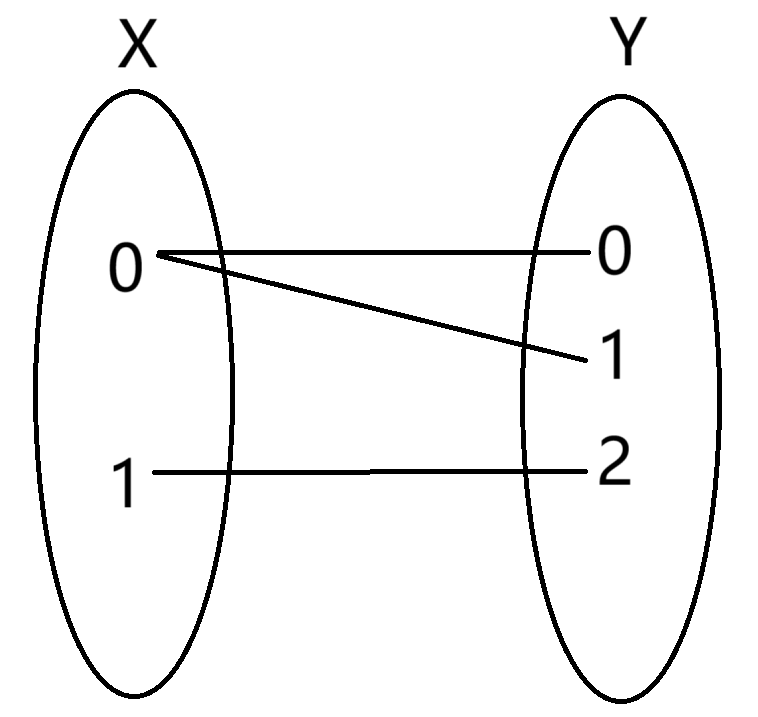
\includegraphics[width=0.45\textwidth]{./figures/chapter1/conditional_entropy_0.png}
\end{figure}
\end{proposition}

\begin{proposition}
Conditioning Reduces Entropy(Information can't hurt):\\
$$H(X)\geq H(X|Y)$$
proof:
\begin{align*}
I(X;Y) &= H(X) - H(X|Y) \geq 0 \\
\Rightarrow H(X) &\geq H(X|Y)
\end{align*}
当且仅当 $I(X;Y)=0$, 即 $X,Y$ 独立时取等.
\end{proposition}

将$X,Y$两个分布的性质拓展到$n$个分布:\\
\textcolor{red}{多元KL散度}:
$$D\left(p(x,y)\|q(x,y)\right)=\sum_{x,y}\textcolor{red}{p(x,y)}\log\dfrac{p(x,y)}{q(x,y)}$$
$$D\left(p(y|x)\|q(y|x)\right)=\sum_{x,y}\textcolor{red}{p(x,y)}\log\dfrac{p(y|x)}{q(y|x)}$$
\textcolor{red}{无论KL散度的形式如何, $\log$前都是$p(x,y)$!!!}

\begin{proposition}
1. Chain Rule:\\
<1> Entropy's Chain Rule:
\begin{align*}
H(X_1,X_2,\cdots,X_n) &= H(X_1) + H(X_2|X_1) + \cdots + H(X_n|X_{n-1},\cdots,X_1) \\
&= \sum_{i=1}^{n}H(X_i|X_1,\cdots,X_{i-1}) \\
&= \sum_{i=1}^{n}H(X_i|X_{i+1},\cdots,X_{n})
\end{align*}

<2> Mutual Information's Chain Rule:
$$I(X_1,X_2,\cdots,X_n;Y)=\sum_{i=1}^{n}I(X_i;Y|X_1,\cdots,X_{i-1})$$
proof:
\begin{align*}
I(X_1,X_2,\cdots,X_n;Y) &= H(X_1,X_2,\cdots,X_n) - H(X_1,X_2,\cdots,X_n|Y) \\
&= \sum_{i=1}^{n}H(X_i|X_1,\cdots,X_{i-1}) - \sum_{i=1}^{n}H(X_i|X_1,\cdots,X_{i-1},Y) \\
&= \sum_{i=1}^{n}\left[H(X_i|X_1,\cdots,X_{i-1})-H(X_i|X_1,\cdots,X_{i-1},Y)\right] \\
&= \sum_{i=1}^{n}I(X_i;Y|X_1,\cdots,X_{i-1})
\end{align*}

<3> KL-Divergence's Chain Rule:
$$D\left(p(x,y)\|q(x,y)\right)=D\left(p(x)\|q(x)\right) + D\left(p(y|x)\|q(y|x)\right)$$
proof:
\begin{align*}
D\left(p(x,y)\|q(x,y)\right) &= \sum_{x,y}p(x,y)\log\dfrac{p(x,y)}{q(x,y)} \\
&= \sum_{x,y}p(x,y)\log\dfrac{p(x)p(y|x)}{q(x)q(y|x)} \\
&= \sum_{x,y}p(x,y)\log\dfrac{p(x)}{q(x)} + \sum_{x,y}p(x,y)\log\dfrac{p(y|x)}{q(y|x)} \\
&= D\left(p(x)\|q(x)\right) + D\left(p(y|x)\|q(y|x)\right)
\end{align*}
$$\Rightarrow D\left(p(x_1,x_2,\cdots,x_n)\|q(x_1,x_2,\cdots,x_n)\right)=\sum_{i=1}^{n}D\left(p(x_i)\|q(x_i)\right)$$


2. Mutual Information $\Rightarrow$ Conditional Mutual Information:\\
$I(X;Y|Z)$: given $Z$, $X$,$Y$的互信息.
\begin{align*}
    I(X;Y|Z) &= H(Y;X|Z) \\
    &= H(X|Z) - H(X|Y,Z) \\
    &= H(Y|Z) - H(Y|X,Z)
\end{align*}
\end{proposition}

已知$H(X)\geq H(X|Y)$, 但是$I(X;Y)$和$I(X;Y|Z)$大小关系不确定.
\begin{example}
$I(X;Y|Z)>I(X;Y)$\\
$X, Y \stackrel{i.i.d.}{\sim} \operatorname{Bern}\left(\dfrac{1}{2}\right)$, $Z=X+Y$\\
$X\perp Y\Rightarrow I(X;Y)=0$
\begin{align*}
I(X;Y|Z) &= H(X|Z) - H(X|Y,Z) \\
&= H(X|Z) \text{\ \ \ (X=Z-Y, deterministic)} \\
&= P(Z=0)H(X|Z=0) + P(Z=1)H(X|Z=1) + P(Z=2)H(X|Z=2) \\
&= 0 + \dfrac{1}{2}H(X|Z=1) + 0 \\
&> 0 \\
I(X;Y|Z) &> I(X;Y)
\end{align*}
\end{example}

\begin{example}
$I(X;Y|Z)\leq I(X;Y)$
Construct Markov Chain: $X\rightarrow Y\rightarrow Z$
\begin{align*}
p(x,y,z) &= p(x)p(y|x)p(z|y) \\
I(X;Y,Z) &= I(Y,Z;X) \\
&= I(Y;X) + I(Z;X|Y) \\
&= I(Z;X) + I(Y;X|Z)
\end{align*}
Since $Z\perp X|Y\Rightarrow I(Z;X|Y)=0$\\
So $I(Y;X)= I(Z;X) + I(Y;X|Z)\geq I(Y;X|Z)$\\
所以$I(X;Y)\geq I(X;Y|Z)$
\begin{align*}
\text{proof:  } Z\perp X|Y &\Rightarrow I(Z;X|Y)=0: \\
I(Z;X|Y) &= H(Z|Y) - H(Z|X,Y) \\
H(Z|X,Y) &= \sum_{x,y,z}p(x,y,z)\log\dfrac{1}{p(z|x,y)} \\
&= \sum_{x,y,z}p(x,y,z)\log\dfrac{1}{p(z|y)}
= \sum_{y,z}p(y,z)\log\dfrac{1}{p(z|y)} \\
&= H(Z|Y) \\
\Rightarrow I(Z;X|Y) &= 0
\end{align*}
\end{example}

\begin{proposition}
$I(X;Y_1,\cdots,Y_n)=\sum\limits_{i=1}^nI(X;Y_i|Y_1,\cdots,Y_{i-1})$\\
$I(X_1,\cdots,X_n;Y_1,\cdots,Y_n)$: 将上面的$X$替换成$X_1,\cdots,X_n$, 然后再展开.\\
Specifically: When $(X_1,Y_1) \perp (X_2,Y_2) \perp \cdots \perp (X_n,Y_n)$, then
$$I(X_1,\cdots,X_n;Y_1,\cdots,Y_n)=\sum\limits_{i=1}^{n}I(X_i;Y_i)$$
\end{proposition}

\begin{example}
我们知道 $H(X)\geq H(X|Y)$, 但是 $H(X)$和 $H(X|Y=y)$的大小不确定. \\
\begin{table*}[!htbp]
    \centering
    \begin{tabular}{c|cc}
        \diagbox{$Y$}{$X$} & $0$ & $1$ \\
        \hline $0$ & $0$ & $\frac{3}{4}$  \\
        $1$ & $\frac{1}{8}$ & $\frac{1}{8}$  \\
        \hline
    \end{tabular}
\end{table*}

\begin{align*}
H(X) &= H\left(\dfrac{1}{8},\dfrac{7}{8} \right)\in \left(0,\log|\mathcal{X}|\right) = (0,1) \\
H(X|Y=0) &= H\left( 0,1 \right) = 0 \\
H(X|Y=1) &= H\left( \dfrac{1}{2},\dfrac{1}{2} \right) = \log|\mathcal{X}| = 1
\end{align*}

\end{example}

\begin{proposition}
从条件熵的角度推导出 cross entropy. 如下图所示, 网络满足马尔可夫链:
$$ Y\rightarrow X\rightarrow Z\to \hat{Y}$$
\begin{figure}[htbp]
    \centering
    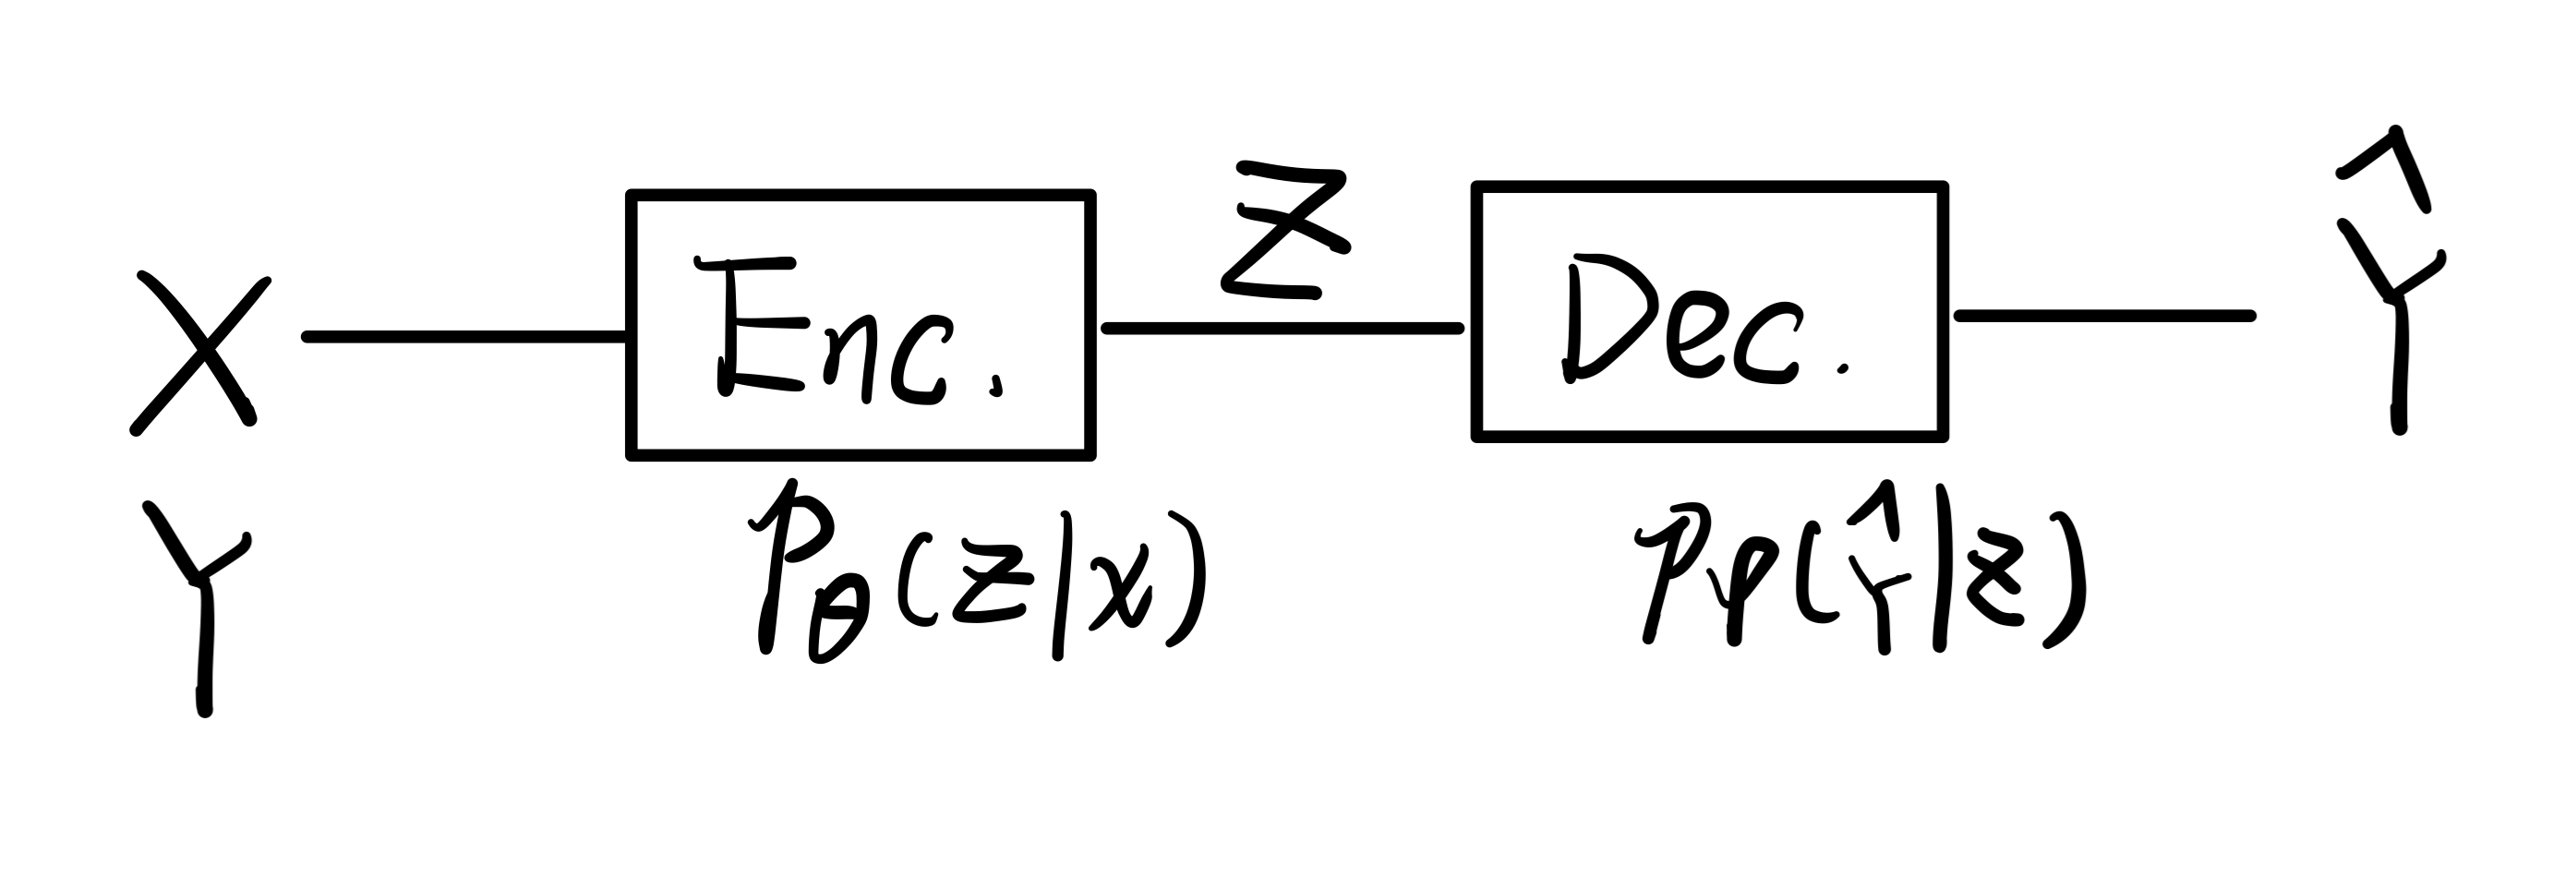
\includegraphics[width=\textwidth]{./figures/chapter1/cross_entropy.png}
\end{figure}
$$\min_{p(\hat{y},z)}\ \ H(\hat{Y}|Z)$$
使网络确定到正确的答案.\\
\begin{align*}
H(\hat{Y}|Z) &= \sum_{\hat{y},z}p(\hat{y},z)\log\dfrac{1}{p(\hat{y}|z)} \\
&= \sum_{x,y,z,\hat{y}}p(x,y,z,\hat{y})\log\dfrac{1}{p(\hat{y}|z)} \\
&= \sum_{x,y}p(x,y)\textcolor{red}{p_{\theta}(z|x)p_{\phi}(\hat{y}|z)}\log\dfrac{1}{p(\hat{y}|z)} \text{\ \ \ (Monte\ Carlo\ sample $\rightarrow (x,y)$)}
\end{align*}
红色部分为网络 trainable的部分, 为了使网络确定到正确的答案, 需要最小化剩余的部分, i.e.
$$\sum_{x,y}p(x,y)\log\dfrac{1}{p(\hat{y}|z)}$$
Which is the cross entropy between $p(x,y)$ and $p(\hat{y}|z)$.
\end{proposition}